\section{Linear Programming}

\subsection{Deductive Reasoning Agents}
Agents that represent the state as logical formulae, and use deductive reasoning to determine the optimal actions. A \emph{Symbolic AI} paradigm. 

\subsubsection{Problems}
\begin{enumerate}
    \item Representation/Reasoning - How does one represent the real world as a set of \\ predicates that are useful?
    \item Transduction - How do we make the translation between the real world and our representation fast enough?
\end{enumerate}

The underlying problem is that symbol-based manipulation is complex and untractable.

\subsubsection{Algorithm}
The agent has a set of rules/predicate statements of the form $state -> action$, where the action is the best action for the given state.\\

At each time step, the agent chooses the rule whose precondition matches the current state. If there isn't a match, it picks the first statement that doesn't contradict the current state. \\

In a static environment, if the agent doesn't have a general rule (base case), it might reach a state where it doesn't know what to do - in this case it will stall. This doesn't mean that the goal is impossible, but that the agent doesn't know how to achieve it. 

\subsection{Planning Agents}
Rather than solving the theorem at each state, the planner makes a plan (sequence of actions), that progresses from the initial state to the goal.

\subsubsection{Problems}
\begin{enumerate}
    \item Representation/Reasoning - How does one represent the real world as a set of \\ predicates that are useful?
    \item Assumes a static environment
    \item First-order logic can be NP-complete
\end{enumerate}

\subsection{Calculative Rationality}
Any agent makes the optimal choice for the state in which it started to make the choice - in dynamic/multi-agent environments, this state might have changed before the decision is made. Such an agent has \emph{calculative rationality}. 
Therefore, an optimal agent needs to be able to plan for the future while reacting to the current state. To represent this, we can use \emph{Temporal Logic}

\subsection{Temporal Logic}

\subsubsection{Symbols}
\begin{figure}[H]
    \centering
    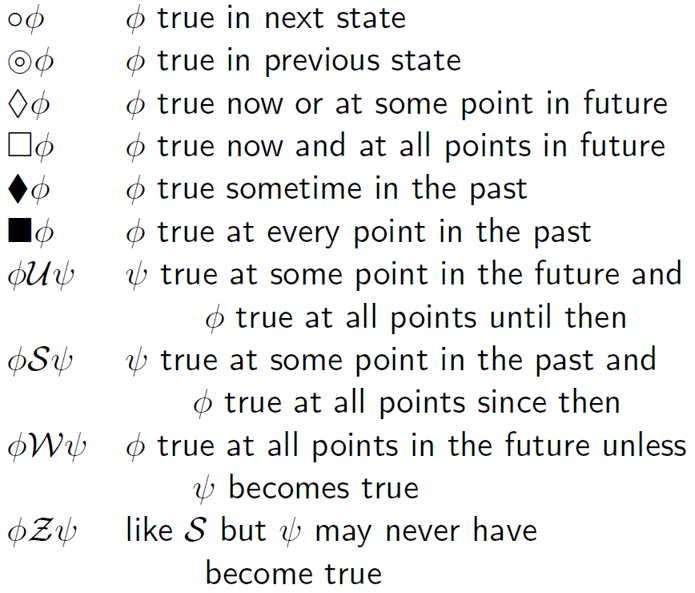
\includegraphics[width = \textwidth]{Images/Temporal_Logic_Symbols}
\end{figure}

\subsubsection{Concurrent MetateM}
\begin{itemize}
    \item Agents are specified as a set of temporal logic rules, permitted incoming arguments, and output types
    \item Each agent uses its history/incoming information to match against rules - on a match, it performs an action
    \item Concurrent agents can communicate with asynchronous messages
\end{itemize} 

At each state, the agent:
\begin{enumerate}
    \item Reads incoming messages to set state booleans
    \item Checks which rules fire in the current state
    \item Executes rules and fulfils any commitments from actions in previous states (commitments take priority)
\end{enumerate} 

This way, the agent separates immediate reactions with long term actions to achieve a goal. The reasoning is still difficult, as is translating the world to symbols. 

\subsection{Brookes: Subsumption Architecture}

\subsubsection{Concept}
This approach is heavily inspired by \emph{Behaviourism}, that a system can be described by how it reacts to its environment. 

It's primary principle is that real intelligence \textbf{must be situated in the real world}, and emerges from the interactions with the world. It can't be achieved by an abstract theorem solver.

Brookes put forward three theses:
\begin{enumerate}
    \item Intelligence can be generated without explicit representations
    \item Intelligence can be generated without abstract reasoning
    \item Intelligence is an emergent property of a complex system, rather than inherent/quantifiable
\end{enumerate}

\subsubsection{Composition}
The architecture is composed of sets of modules/rules/behaviours, each of which takes the form:
\begin{center}
    IF situation THEN action
\end{center}
These behaviours are organised into hierarchies to resolve ties. 

\subsubsection{Performance}
Though simple, it achieves near-optimal performance on multiple domains. However, it can't think ahead to future episodes, and doesn't have a history to reference. 

\subsection{Hybrid Architectures}
Some researchers have suggested an agent with two subsystems: one deliberative, one reactive. Usually the reactive takes priority.

To manage priorities, the system is split into layers:
\begin{description}
    \item[Horizontal Layering] Each layer is connected to the input and output, and each gives a separate suggestion - as if each were a separate agent
    \item[Vertical Layering] Layers are connected to each other (one connected to input, one to output), and take the results from the previous layer as input to make decision
\end{description}

Horizontal layering gives a wide variety but introduces a bottleneck as every layer must wait for the slowest. Vertical layering isn't tolerant to a single layer failing, but makes decisions across multiple layers than a single choice at the end. 
